\documentclass[10pt]{article}
\usepackage[margin=1in]{geometry}
\usepackage{amsmath,amssymb,graphicx}
\usepackage[hidelinks]{hyperref}
\title{SkewKeeper: Bounded Temporal Synchronization\\for Parallel Full-System Emulation}
\author{Author information pending}
\date{Draft: September 2026 --- Evaluation pending}
\newcommand{\todo}[1]{\par\noindent\textbf{TODO:} #1\par}
\begin{document}
\maketitle
\begin{abstract}
Parallel full-system emulation can expose a mismatch between guest execution
progress and a host-driven virtual clock. SkewKeeper introduces per-vCPU logical
instruction progress, a coordinator based on the slowest active member, and a
bounded execution window. A shared visible clock interpolates between model
updates while limiting its deviation from instruction-derived time. We describe
a QEMU 10.2.0 prototype and a hardware-calibration methodology for functional
timing. The current artifact contains an experimental protocol, validated data
formats, and figure-generation tools. Hardware equivalence, deadline preservation
under host throttling, and scaling benefits remain evaluation questions; this
draft reports an initial visible-time study; the other experiments remain planned.
The study also identifies a wide-IPS conversion defect.
\end{abstract}

\section{Introduction}
Functional emulation enables unmodified system software to run on a different
host architecture. QEMU uses dynamic translation for this purpose
\cite{bellard2005}. Parallel execution increases the usefulness of full-system
emulation, but execution progress and software-visible time must remain meaningfully
related. If a guest deadline advances with host time while translated processing
takes longer than on the target hardware, an emulated workload may miss a deadline
that hardware would meet.

SkewKeeper assigns a logical time scale to executed guest instructions and
constrains how far a fast vCPU can lead shared progress. Its goal is a
hardware-calibrated functional-time approximation, subject to calibration across
representative workloads. It does not model cycles, caches, pipelines, or memory
stalls. Instruction progress supplies a stable conversion rule; the instruction
sequence and multicore schedule themselves need not be invariant under host load.

The proposed contributions are (1) epoch-based logical progress with explicit
idle membership, (2) a bounded parallel execution window using common TB-budget
machinery, (3) a shared, bounded visible-time interpolator, and (4) a reproducible
calibration and evaluation methodology. Hardware-calibrated accuracy is an
objective of the methodology, not an established result.

\section{Background and Motivation}
\subsection{Parallel TCG and instruction counting}
Upstream MTTCG executes supported vCPUs in distinct host threads. Icount instead
requires the single-thread execution path; it can simulate an SMP guest without
parallel vCPU execution \cite{qemumttcg,qemuicount}. Fixed-shift icount derives time
from instruction counts, while adaptive modes can adjust the conversion.
Instruction counting is not a microarchitectural timing model.

\subsection{Virtual clock and system counter}
In this prototype, the Arm generic timer obtains time from
\texttt{QEMU\_CLOCK\_VIRTUAL} and converts nanoseconds into counter ticks. The
virtual-counter offset and counter frequency still apply. A guest
\texttt{CLOCK\_MONOTONIC} read depends on its selected clocksource and kernel
timekeeping path; it is not universally a direct counter instruction.
Devices using this virtual clock also observe the prototype's visible clock.

\subsection{Illustrative deadline mismatch}
Consider a communication-processing ROI with hardware completion time $T_h$ and
deadline $D>T_h$. On a slower emulator it may consume host time $T_e>D$ even
without a guest logic error. A host-driven clock may therefore report a miss.
This is a motivating construction, not measured evidence. A fixed-scale
host-clock comparator could compensate for one speed ratio but would retain
host-speed dependence. No such comparator is claimed to exist in the current
artifact; its implementation must be identified before comparison.

\section{Design}
\subsection{Logical instruction progress}
For CPU $i$, let $R_i$ be its accumulated executed-instruction count,
$R_i^0$ the raw count at the current membership epoch, and $L_i^0$ its logical
base. Define
\[
 L_i=L_i^0+(R_i-R_i^0).
\]
Raw progress is retained across idle periods. On re-entry, setting
$R_i^0=R_i$ and $L_i^0=G$ aligns the CPU with current shared progress.
This changes the mapping, not the number of physically executed instructions.

\subsection{Active membership and global progress}
Let $A$ denote the participating active set. While $A$ is nonempty,
\[
 C=\min_{i\in A}L_i,\qquad G\leftarrow\max(G,C).
\]
The coordinator observes published counts; it does not read an instantaneous
instruction boundary on every CPU. Stop and actual idle predicates remove
members. A window waiter remains active, preventing fast CPUs from advancing
global time alone. A WFE instruction cannot by itself be assumed to remove a CPU.

With no active members and all CPU threads idle, the coordinator commits the
maximum completed tail before applying a virtual-timer warp. This preserves
executed work at the end of an epoch. Inactive CPUs can retain historical logical
values below $G$ until re-entry; the active lower-bound statement does not apply
to them.

\subsection{Execution window and dispatch budget}
Let $W$ be the configured instruction window and $\ell_i=L_i-G$ the active lead.
The intended active invariant is $0\leq\ell_i\leq W$. A dispatch loads
\[
 B_i=\min(65535,\ W-\ell_i).
\]
The 16-bit chunk is a representation limit, whereas $W$ expresses allowed
divergence. A TB entry checks whether the complete block fits; an insufficient
budget returns to the CPU loop, which can request a shorter TB. Exhaustion
aggregates into the common CPU exit path. The MTTCG thread accounts completed
work and waits at the window boundary using the existing scheduling flow.

Under a consistent observation of all active $L_i$ and $G$, the lead invariant
implies $\max_{i\in A}L_i-\min_{i\in A}L_i\leq W$. Sampled publications alone do not
prove this invariant for every in-flight instruction. Exception paths and atomic
retries require accounting tests.

\begin{figure}[ht]
\centering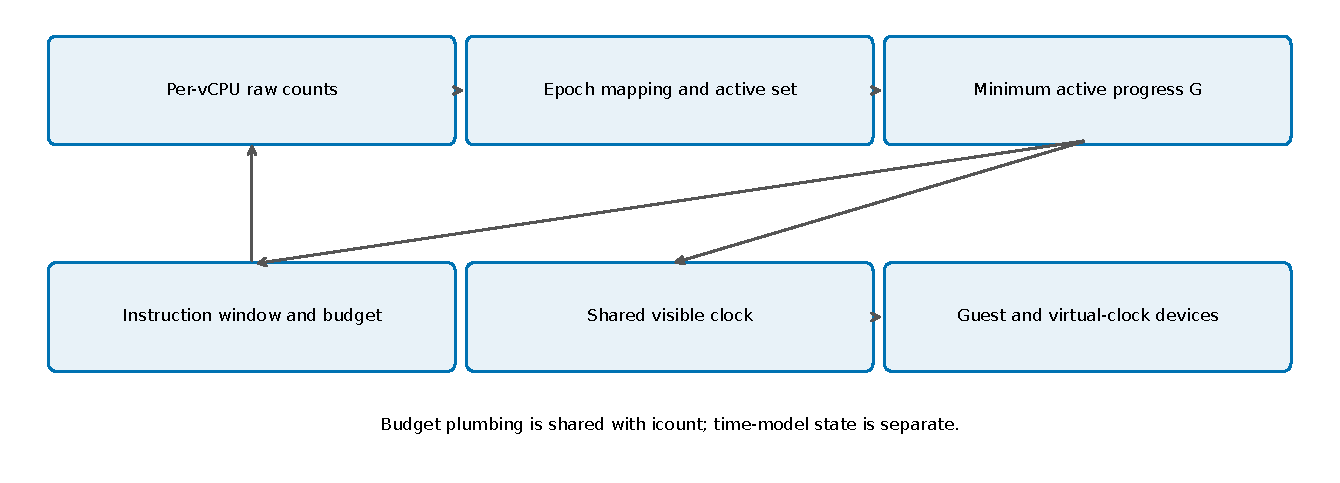
\includegraphics[width=\linewidth]{figures/design/D1-architecture.pdf}
\caption{Mechanism schematic, not an experimental result.}
\end{figure}
\begin{figure}[ht]
\centering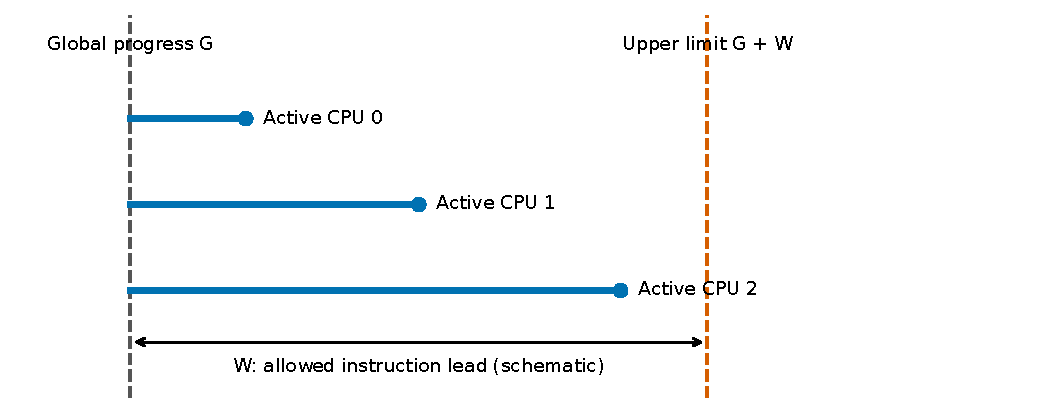
\includegraphics[width=.85\linewidth]{figures/design/D2-window.pdf}
\caption{Active progress and window. Idle histories are rebased on re-entry.}
\end{figure}

\subsection{Strict model time}
For configured instructions per simulated second $S$,
\[
 M=O+H+\left\lfloor G\,10^9/S\right\rfloor,
\]
where $O$ is the accumulated epoch offset and $H$ is idle-warp time. For a fixed
instruction delta in an unchanged epoch, the instruction-derived increment is
independent of host elapsed time. Idle transitions, I/O, and different guest paths
can still change elapsed model time. Budget generation is window based; there is
no separate model-only device-timer domain in this prototype.

\subsection{Visible-time interpolation}
Let $a$ be a shared visible anchor, $h_a$ its pause-aware host-clock anchor, and
$s$ the stored slope. A read at $h$ computes
\[
 P=a+s\max(h-h_a,0),\quad
 B=\min(\max(P,\max(M-w,0)),M+w),
\]
and publishes a nondecreasing shared value using an atomic maximum, where $w$
is the window in nanoseconds. Coordinator re-anchoring also clamps against the
new model bounds. Cross-thread publication races must be audited in addition
to checking the arithmetic formulas.

At update $k$, actual elapsed interval $\Delta h_k$ and instruction delta
$\Delta G_k$ form
\[
 d_k=\min(\Delta G_k,\lfloor S\Delta h_k/10^9\rfloor),\qquad
 r_k=\frac{\lfloor d_k10^9/S\rfloor}{\Delta h_k}.
\]
The most recent eight samples are averaged with weights $(3/4)^j$. The
implementation uses Q32 arithmetic and a clipped feedback correction
$0.01\min(|V-M|/\Delta h_k,1)$, subtracting it when visible time leads.
Active execution imposes a slope floor $1/256$; idle intervals use zero.
An idle-to-active transition may reset the interpolation anchor before the
next coordinator callback.

Stored slopes lie in $[0,1]$, but this is not a bound on forward jumps caused by
re-anchoring or idle warp. When a read reaches $M+w$, its returned value plateaus;
it does not change the stored slope. Slope mutation on a bound-hit read is
an unimplemented extension. The clock is piecewise linear between updates,
with quantization and possible saturation, rather than strictly continuous.
A finite bound and stalled model cannot support indefinitely increasing time.

\begin{figure}[ht]
\centering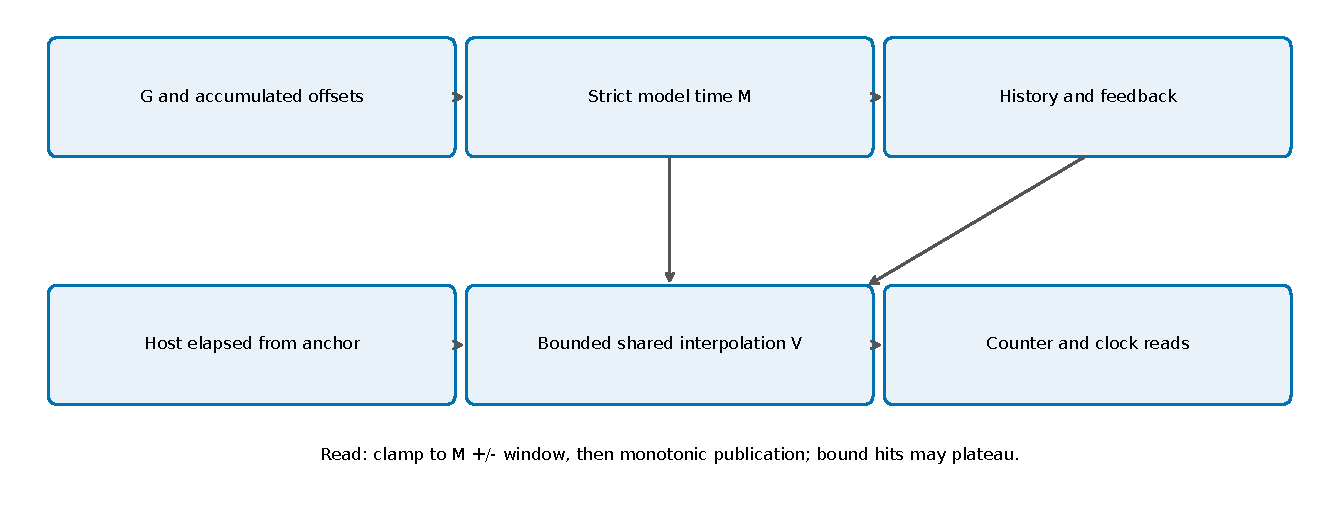
\includegraphics[width=\linewidth]{figures/design/D3-time-path.pdf}
\caption{Strict progress and shared visible time. Host elapsed time enters the
interpolator, so exact host-speed independence is not claimed.}
\end{figure}

\subsection{Calibration method}
For a matched serial ROI with executed instructions $I$ and measured target
hardware time $T_h$, equivalent IPS is $I/T_h$. A single $S$ is selected on a
calibration set and evaluated on held-out workloads. Parallel model time depends
on global progress, not the sum of all CPU instruction counts, so those metrics
must not be interchanged. The method approximates functional timing within a
workload family; transferring it across instruction mixes is an experimental
question.

\section{Implementation}
The prototype is based on QEMU 10.2.0, revision
\texttt{4e894601b8} \cite{skewsource}. The implementation centers on
\path{accel/tcg/skew.c}. CPU state stores raw counts, epoch bases, membership
and budget state. \path{include/exec/exec-budget.h} supplies shared budget
operations, while independent icount and skew adapters manage their own time
models. \path{cpu_loop_exec_tb} handles common execution exits;
\path{mttcg_cpu_thread_fn} performs skew prepare/account/wait steps.

A realtime coordinator callback runs under the BQL, samples progress, manages
idle warp and wakes waiters. Reads use a sequence lock for interpolation
parameters and atomic publication of shared visible time. QMP exposes model
time, visible bias, slope and published CPU state, useful for coarse observation.
It does not provide a complete trace of guest counter reads. Optional QMP
MTTCG/skew switching is retained but is not required by this design's
continuous-skew experiments. Migration and snapshots remain blocked because
the prototype lacks a complete state-transfer protocol.

\section{Evaluation: Plan and Initial Visible-Time Study}
Experiments 1--4 remain planned. The explicitly synthetic example CSVs are used
only to test plotting and are excluded from this paper. Section 5.4 reports
separately archived measurements from experiment 5 on September 20, 2026.

\subsection{RQ1: Hardware-equivalent timing and host capacity}
Experiment 1 measures paired hardware ROI time and guest instruction counts,
selects one IPS on calibration workloads and reports held-out relative errors.
Required statistics are mean, median and maximum absolute relative error,
signed-error standard deviation and per-workload results.
\todo{Obtain target-hardware traces, freeze the split and calibration, then populate E1--E2.}

Experiment 2 fixes workload/configuration and varies a dedicated cgroup CPU
quota across 100, 80, 60, 40 and 20 percent of a fixed CPU allocation. Plain
MTTCG, fixed-shift icount and skew are compared; fixed-scale slowtime is optional
and requires a documented implementation. Record host elapsed, guest elapsed,
model elapsed and all deadline outcomes. Failed attempts remain in the miss-rate
denominator. Quota throttling and actual CPU usage must be logged.
\todo{Run controlled repetitions and populate E3--E4. Do not infer deadline
preservation from shorter or longer host completion time alone.}

\subsection{RQ2: Parallel performance}
Experiment 3 evaluates 1, 2, 4 and 8 vCPUs, plus topology-specific counts.
Measure completion time and instruction throughput on uniform, uneven, memory,
idle/re-entry and mixed work. Separate fixed-total strong scaling from
fixed-per-CPU throughput scaling. Normalize each method to its own one-vCPU run.
\todo{Collect at least seven repetitions per cell and populate E5--E6.}

\subsection{RQ3: Window trade-off}
Experiment 4 varies instruction window from $10^3$ to $10^7$, reporting actual
rounded configuration, throughput, sampled active spread, maximum sampled lead,
wait-entry rate and separately observed budget exits. In-flight skew requires
stronger instrumentation than asynchronous QMP snapshots.
\todo{Measure instrument overhead, preserve bound violations and populate E7--E9.}

\subsection{Visible-time validation}
Experiment 5 requires ordered joint records of host time, model time, global
progress, visible time, counter ticks, coordinator events and software reads.
Plot raw segments and steps, never a fitted curve. Report backward steps, bound
violations, repeated counter values, bias and successive-read delta variance.
Include coordinator delay, idle re-entry, pause/resume, high IPS and saturation.
Jitter initialization and sustained use test availability, not entropy quality.
\paragraph{Method.}
We reused the AArch64 bare-metal boot harness and Linux jitter test. An independent
experiment binary reused the existing build objects except for copied skew and
Arm counter-helper sources. The production binary and source were unchanged.
Counter callbacks recorded actual returned ticks together with the corresponding
model, visible value and stored slope in a preallocated buffer under the existing
BQL; the buffer was written at exit. Paired uninstrumented runs checked guest
counter monotonicity. The host was WSL2 Ubuntu 20.04 on x86-64; the guest counter
frequency was 62.5 MHz. Full environment and binary hashes are archived.

Eleven scenarios each used one warmup and seven formal runs per binary, yielding
154 formal executions and 392,000 instrumented counter reads. All guest executions
completed. Collected counter/visible values had no backward steps or window
violations, with no dropped or unlocked records. Each returned counter matched
the recorded visible nanoseconds divided by 16. Two CPUs alternated reads using
a release/acquire handshake in the cross-CPU scenario.

\paragraph{Repeated reads and saturation.}
Across seven runs, the median fraction of identical consecutive counter reads
was 22.181\% in the steady scenario, 94.999\% in the dense scenario and 8.752\%
with alternating CPUs. For unchanged model values in these same traces, the
fractions were 99.750\%, 100\% and 99.450\%, respectively. This diagnostic does
not replace an independently executed ablation with interpolation disabled.
A frozen model has zero delta variance; that alone does not establish clock quality.

To force saturation, the experiment copy delayed each counter callback by
100 microseconds while retaining the existing BQL. With 2G IPS, a 10-microsecond
window and 100-millisecond coordinator interval, 27,699 of 28,000 formal reads
hit the upper bound; 27,678 adjacent pairs formed observed plateaus at unchanged
model time. All bound-hit records retained a positive stored slope. This validates
clamping behavior under explicit fault injection, not natural-workload performance.

\begin{figure}[ht]
\centering

\includegraphics[width=.95\linewidth]{experiments/exp5_visible_time/results/20260920/figures/saturation-onset/E10-visible-timeline.pdf}
\caption{Measured onset of saturation at 2G IPS. Software counter reads reach the
10-microsecond upper bound while the model remains fixed. The experiment injects
a 100-microsecond delay before each read; plotted points are recorded values.}
\end{figure}

\paragraph{A failed invariant at wide IPS.}
Sustained 20G-IPS runs failed the configured model-time formula in all seven
repetitions, although the clock remained bounded and nondecreasing. The QEMU
\texttt{muldiv64} helper accepts 32-bit multiplier and divisor arguments; passing
the 64-bit configured IPS truncates values above $2^{32}-1$. A production-binary
QMP check returned a 2,820,130-instruction window for 20G IPS and a 1ms window,
rather than 20,000,000. The effective truncated IPS was 2,820,130,816. All 12,099
nonzero-global samples in the selected sustained run matched this truncated
conversion and failed the nominal one. Initial 20G saturation runs also failed
the model formula and remain in the archive; the 2G saturation study above avoids
that defect. Short 20G traces ending before global progress advanced could not
detect the formula error. These pre-fix failures remain archived separately.

\paragraph{Wide-IPS correction and regression.}
A subsequent fix uses 64-bit operands and a 128-bit intermediate for window,
model-time and momentum conversions, saturating unrepresentable results.
Eight QMP configurations, including $2^{32}$ and the supported maximum of
$10^{12}$ IPS, now return the expected window. Forty-four arithmetic cases also
cover coordinator intervals beyond $2^{32}$ nanoseconds. Seven new scenarios
with seven formal repetitions per binary passed all 98 executions, including
sustained 20G IPS, the 32-bit boundary, the supported maximum, saturation and
cross-CPU reads. The 336,000 instrumented reads had no model-formula,
counter-conversion, monotonicity or bound violations. This corrects conversion
width; it does not eliminate saturation plateaus or guarantee entropy quality.

\paragraph{Reuse and limits.}
Seven formal Linux boots at 2G IPS passed jitter initialization and 256 actual
64-byte AF\_ALG jitterentropy reads each, with skew enabled from reset. Existing
quick acceptance tests for pause, idle/IRQ, instruction accounting and CPU control
also passed. These results do not certify entropy quality or all concurrency
interleavings. Non-injected probe/baseline process-time ratios were approximately
1.02--1.06 for short scenarios and 1.00--1.01 for sustained ones, including startup
and log output; they are not isolated per-read costs. The model-only ablation and
broader workload validation remain pending.


\section{Limitations and Threats to Validity}
Constant IPS omits microarchitectural effects and may not generalize across
workloads. Active membership, interrupts and external communication can change
the instruction trajectory. Visible time explicitly uses host elapsed intervals;
at high IPS, the active slope floor may exceed model progress and saturate at
the window bound. Quantized counters can repeat even with a positive slope.
Bounded error therefore does not imply every read advances or all deadline
failures disappear.

The publication invariant also requires concurrency analysis: a read-side atomic
maximum and a coordinator store must not overwrite a more recent observation.
Finite sampling and successful boot tests cannot replace that audit. We report
this as an open verification obligation rather than a proved theorem.
Existing host benchmarks are not imported automatically because their versions,
work definitions and timing models may differ from the evaluation protocol.

\section{Related Work}
QEMU's original paper describes its dynamic translation approach
\cite{bellard2005}. The current upstream documents explain separate MTTCG and
icount mechanisms \cite{qemumttcg,qemuicount}. SkewKeeper reuses execution-budget
plumbing while adding active-set progress and shared bounded interpolation.
\todo{Extend the verified literature survey on conservative parallel simulation,
virtual time and functional timing before making novelty claims.}

\section{Conclusion}
SkewKeeper implements instruction-based coordination and a bounded shared
visible clock within parallel full-system emulation. The artifact defines how
to evaluate hardware calibration, host-capacity sensitivity, parallel performance
and synchronization cost. Initial visible-time measurements support bounded,
nondecreasing behavior in the tested scenarios and expose a wide-IPS conversion
defect. Hardware-calibration and parallel-performance claims await further measurements.

\bibliographystyle{plain}
\bibliography{references}
\end{document}
